\documentclass{article}
\usepackage[utf8]{inputenc}
\usepackage[spanish]{babel}
\usepackage{listings}
\usepackage{graphicx}
\graphicspath{ {images/} }
\usepackage{cite}

\begin{document}

\begin{titlepage}
    \begin{center}
        \vspace*{1cm}
            
        \Huge
        \textbf{Parcial II 2021-1 Informática 2}
            
        \vspace{0.5cm}
        \LARGE
        Informe de Análisis y Diseño de la Solución del Desafío
            
        \vspace{1.5cm}
            
        \textbf{Juan Diego Cabrera Moncada}\\
            
        \vfill
            
        \vspace{0.8cm}
            
        \Large
        Despartamento de Ingeniería Electrónica y Telecomunicaciones\\
        Universidad de Antioquia\\
        Medellín\\
        Septiembre de 2021
            
    \end{center}
\end{titlepage}

\tableofcontents
\newpage
 \section{Análisis del problema y consideraciones para la alternativa de solución propuesta}
 En esta fase de análisis, al reconstruir el código que se había propuesto en clase, pude verificar que entendía en su totalidad el método de obtención de la información de cada pixel de una imagen en específico.
 \begin{figure}[h]
    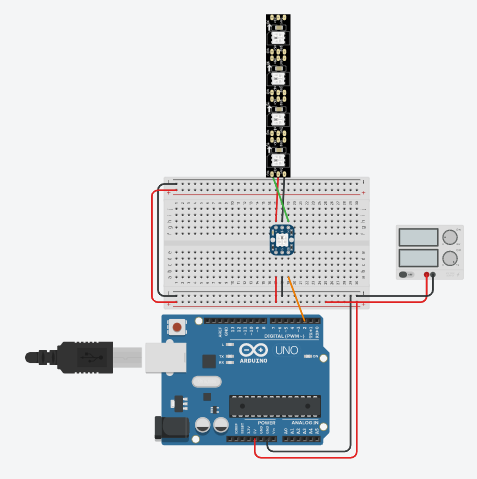
\includegraphics[width=10cm]{circ_pruebainicial.png}
    \centering
    \caption{Réplica del circuito propuesto en clase}
    \label{fig:replica_circInicial}
 \end{figure}
 Posterior a ello, asumí que el mayor problema en la programación sería hacer una función con la cual hiciese el proceso de submuestreo de una imagen, y otra similar, que hiciese el de sobremuestreo, en caso de que alguna de las dos sea necesaria. Para ello, en primer lugar, enfocándome en el submuestreo, pensé en que si obtenía el cociente de la división del ancho de la imagen entre el número de columnas de la matriz de Neopixeles o de LEDs, y de forma similar el alto entre el número de filas, para, posteriormente, usar dichos dos valores (Llamémoslos Cx y Cy), para hallar el promedio de un número Cx de valores (Teniendo en cuenta que pueden ser diferentes dependiendo de cúal de los 3 colores RGB esté analizando matricialmente) y así reducir ese número Cx a 1, y unir todas los valores resultantes hasta crear la versión submuestreada de la matriz. No obstante, al consultar opiniones al respecto en foros y otros sitios web, encontré que esto puede resultar inefectivo por cuestiones de que, hablando de un solo punto de la matriz, la distancia que habría entre los puntos de la matriz real que debe representar el punto de la matriz de submuestreo implica que unos puntos tengan más "peso" que otros al momento de hacer este proceso \cite{AplicarRemuestreo}. No obstante, uno de los comentarios \cite{Comm_ReduImg} proponía hacer el promedio de modo que se haga un submuestreo de reducir la matriz a la mitad en cada ejecución de la función, y, una vez se encuentre cerca de la matriz deseada, hacer la consideración de la influencia que tendría la distancia relativa entre un punto de la matriz real y el punto de la matriz de submuestreo que lo representa. He decidido optar por una matriz de 8 x 8 usando 8 tiras de 8 Neopixeles cada una. Por el momento, procedo a hacer una verificación de que el funcionamiento del código y el circuito está bien planteado para una matriz de Neopixeles de esta cantidad.
 \begin{figure}[h]
    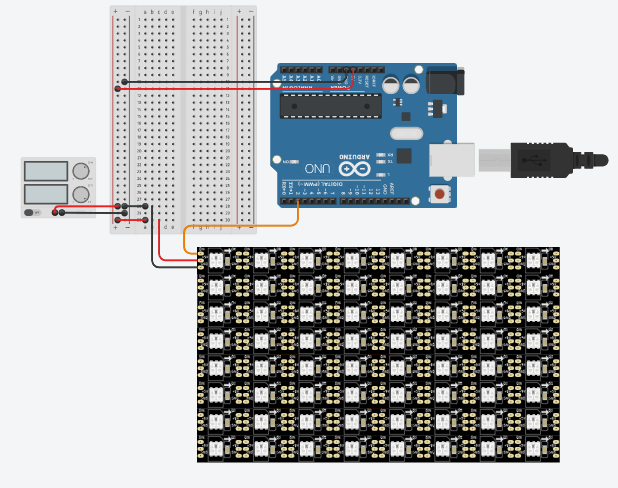
\includegraphics[width=10cm]{matriz8x8Neopixeles.png}
    \centering
    \caption{Construcción de matriz 8x8 de Neopixeles}
    \label{fig:matriz8x8Neopixeles}
 \end{figure}
Al analizar detenidamente la matriz de Neopixeles y después de unas cuantas pruebas en código, considero que el algoritmo debe fundamentarse en el manejo de dos clases principalmente, una de ellas que debe encargarse, a través de sus métodos, de poder leer cada uno de los pixeles que componen a la imagen cuya dirección ingrese el usuario en el programa en Qt, así como, de ser necesario, poder usar métodos que permitan obtener el valor de cada color (Rojo, verde y azul) y modificarlos si así lo plantea la implementación del algoritmo. La segunda clase debe encargarse de guardar los datos acerca de los valores enteros de rojo, azul y verde que debe adquirir individualmente cada neopixel, los cuales son obtenidos después de haber procesado la imagen, ya sea por submuestreo o sobremuestreo de la misma. Dicha clase debe garantizar que se pueda acceder a dichos valores enteros de manera eficiente con el objetivo de escribir dichos valores en un archivo de texto bajo un formato preestablecido. En cuanto al programa en Tinkercad, considero que esta alternativa de solución debe permitir que los datos del archivo de texto sean leídos y guardados en una matriz de variables tridimensional, considerando que se trata de valores enteros para 3 colores diferentes, que deben ser representados en una matriz de 8 columnas por 8 filas. Asimismo, a través de las funciones del programa, se debe usar una librería que permita la configuración del valor del color de los neopixeles en formato RGB (Rojo, verde y azul), de modo que los valores enteros guardados anteriormente en la matriz tridimensional se usen como referencia para configurar los neopixeles que conforman la matriz de 8 x 8 de tiras de Neopixeles.
Otra alternativa de solución posible, la cual fue considerada a último momento, consiste en considerar la imagen como un conjunto de figuras geométricas, lo cual, en una imagen normal costaría mucho espacio en memoria, pero al tratarse de una bandera, la cantidad de figuras a considerar son más bien pocas, por lo cual es posible analizarla de dicha forma. Por este método, se considera cada figura como una unión de pixeles del mismo color, de tal modo que si una vez se lea que el pixel inmediatamente al que donde uno se encuentra es de diferente color, implica que ese es uno de los bordes de la figura. De este modo, cuando una figura de un mismo color no representa un porcentaje lo suficientemente alto como para ser representada en una matriz de 8 x 8, simplemente se ignora dicha figura y se toma la figura predominante que encierra a dicha figura. Tome como ejemplo las estrellas de la bandera de estados unidos, al ser tan pequeñas como para ser representadas una a una dentro de una matriz de 8 x 8 (A menos que la imagen dada de la bandera tenga las estrellas lo suficientemente grandes), simplemente se ignora la representación de las mismas o, dado el segundo caso, se intercala entre azul y blanco para su representación. En cuanto a banderas que contienen letras o escudos, esta segunda alternativa implica que sólo se considere el color más predominante dentro de la imagen, por lo cual, por ejemplo, si las letras están contenidas dentro de un rectángulo blanco, sólo se tome en consideración el rectángulo blanco al representar la bandera en la matriz. Asimismo, para el caso de los escudos, al ser de distintos colores en un sólo lugar, se analiza el color de mayor predominancia para tener dicho color en principal consideración para representar el escudo en la matriz de neopixeles, y en caso de ser varios colores los que predominan, se hace un promedio de los mismos para obtener el resultado. Cabe destacar que se busca que esta segunda alternativa de solución sea implementada únicamente en caso de que la primera falle y, de ser posible si la primera no es lo suficientemente efectiva, combinar ambas de tal modo que, en primer lugar, se usa el concepto de interpolación bilineal para reducir el tamaño de la imagen hasta cierto punto, y después analizarla por el segundo método, o viceversa. Así, se busca que el esquema de tareas se vea inalterado así como las clases implementadas, el manual de uso y las consideraciones en la implementación sean las mismas, dado que ésta segunda alternativa de solución solo implica afectar el algoritmo planteado para el programa en Qt, más no el programa en Tinkercad, el cual sólo ha de estar basando su lógica de planteamiento en el formato preestablecido para el archivo de texto que contiene la información sobre lo que debe representar cada neopixel de la matriz, además de considerar el uso de métodos y funciones para recibir dicha información, guardarla y adjudicársela a cada neopixel de manera efectiva. Asimismo, en Tinkercad es fundamental considerar el uso de una librería que permita la configuración de dichos neopixeles, sea cual sea el algoritmo final planteado para la parte de Qt.
 \section{Esquema de tareas del desarrollo del algoritmo}
 En primer lugar, procedo a analizar la lista de tareas que se deben ejecutar para desarrollar el algoritmo de solución del desafío de manera efectiva. Analizando objetivos de forma secuencial, considero que, primero, es fundamental establecer el método de interacción con el usuario para solicitar la imagen a procesar, por lo cual, una parte de ello, consta de la creación del manual de uso del programa., que debe abordar a su vez, lo que debe hacer el usuario con el archivo de texto resultante del submuestreo o sobremuestreo de la imagen (En caso de que sea alguno de los 2 necesario), incluyendo cómo y dónde debe usarlo, pues dicho archivo contiene la información necesaria para que funcione correctamente la solución implementada en Tinkercad (Primera impresión de cómo debe conectarse Tinkercad y Qt). Una vez hechas las partes de interacción con el usuario, la siguiente tarea corresponde a crear un método de lectura de la información de la imagen y proveer una forma, mediante código, de guardar dicha información de modo que resulte cómoda de usar al procesarla para la cuestión de submuestreo o sobremuestreo de la imagen. Posterior a ello, debo definir métodos que me permitan manipular la información almacenada. Después, es necesario definir métodos, ciclos y ejecuciones necesarias para el caso en que se requiera realizar submuestreo de la imagen, en paralelo con aquellos necesarios para el caso de sobremuestreo de la imagen. Es necesario, después, garantizar métodos así para guardar la nueva información procesada de la imagen en conjunto con la manipulación del archivo de texto. Asimismo, otra tarea fundamental, la cual puede hacerse en paralelo con el proceso anteriormente descrito, radica en la construcción de la matriz de Neopixeles de modo que sea funcional, en primera instancia, y posterior a que ésto se garantice, priorizar la efectividad en la representación matricial de la información procesada de la imagen obtenida por vía del archivo de texto creado y modificado. Esta última tarea, se debe subdividir en la garantización de la representación matricial para cada uno de los colores RGB por separado como primer objetivo y, después, en conjunto.
  \begin{figure}[h]
    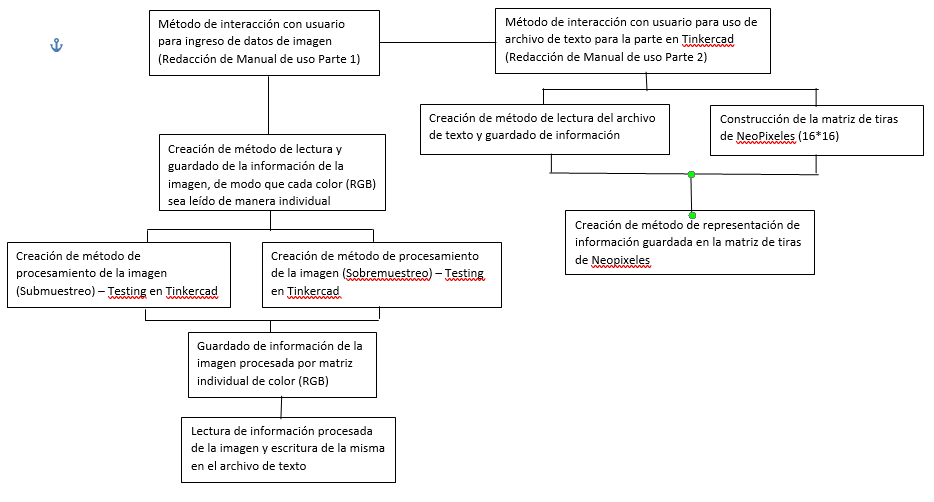
\includegraphics[width=10cm]{Esquema_Tareas.png}
    \centering
    \caption{Esquema de Tareas}
    \label{fig:esquema_tareas}
 \end{figure}
 \section{Diseño del algoritmo}
 El algoritmo diseñado para cumplir con la alternativa de solución planteada en primer lugar es el siguiente:
  \begin{figure}[h]
    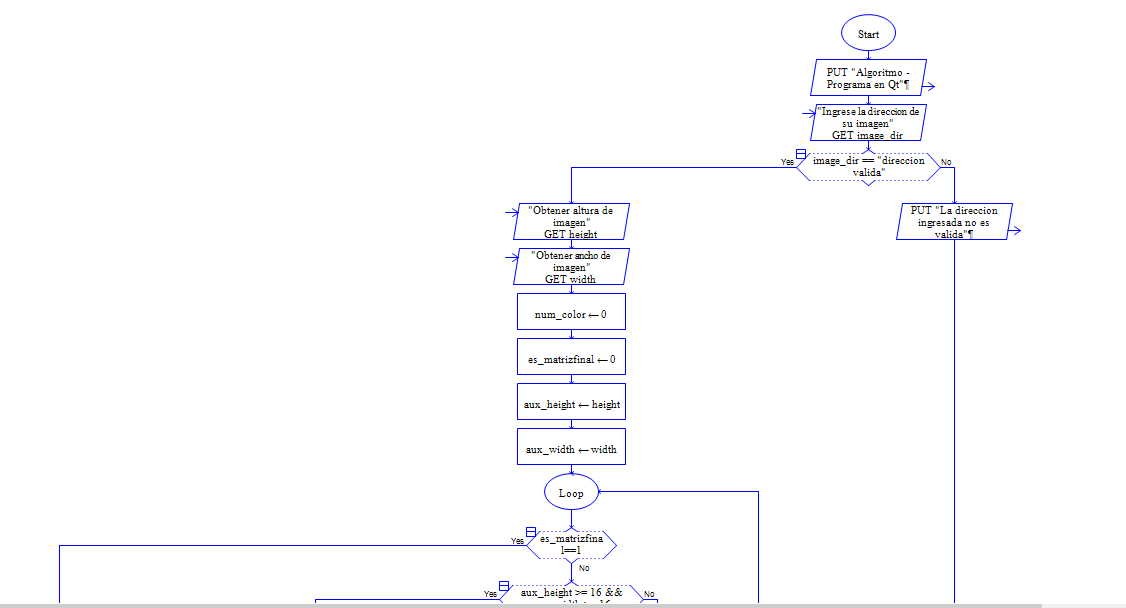
\includegraphics[width=8cm]{flow_1.png}
    \centering
    \caption{Diagrama de Flujo 1}
    \label{fig:flow_1}
 \end{figure}
  \begin{figure}[h]
    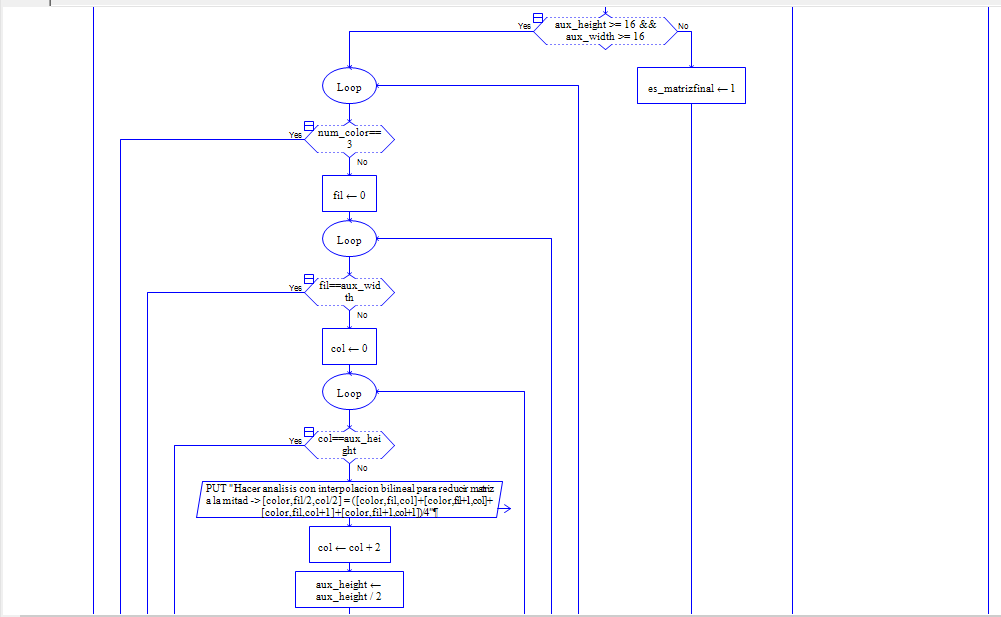
\includegraphics[width=8cm]{flow_2.png}
    \centering
    \caption{Diagrama de Flujo 2}
    \label{fig:flow_2}
 \end{figure}
  \begin{figure}[h]
    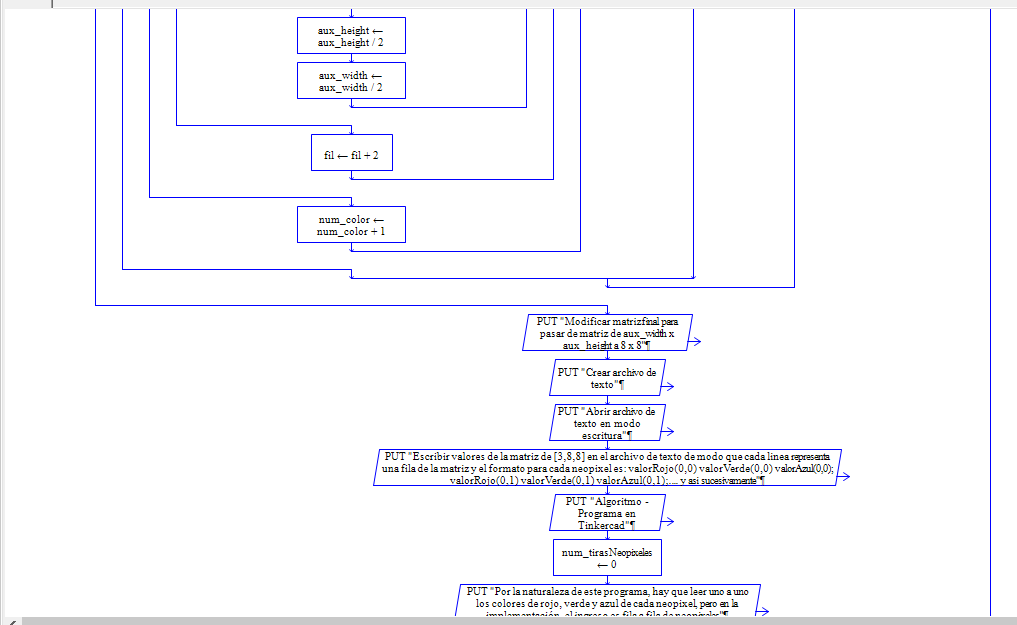
\includegraphics[width=8cm]{flow_3.png}
    \centering
    \caption{Diagrama de Flujo 3}
    \label{fig:flow_3}
 \end{figure}
  \begin{figure}[h]
    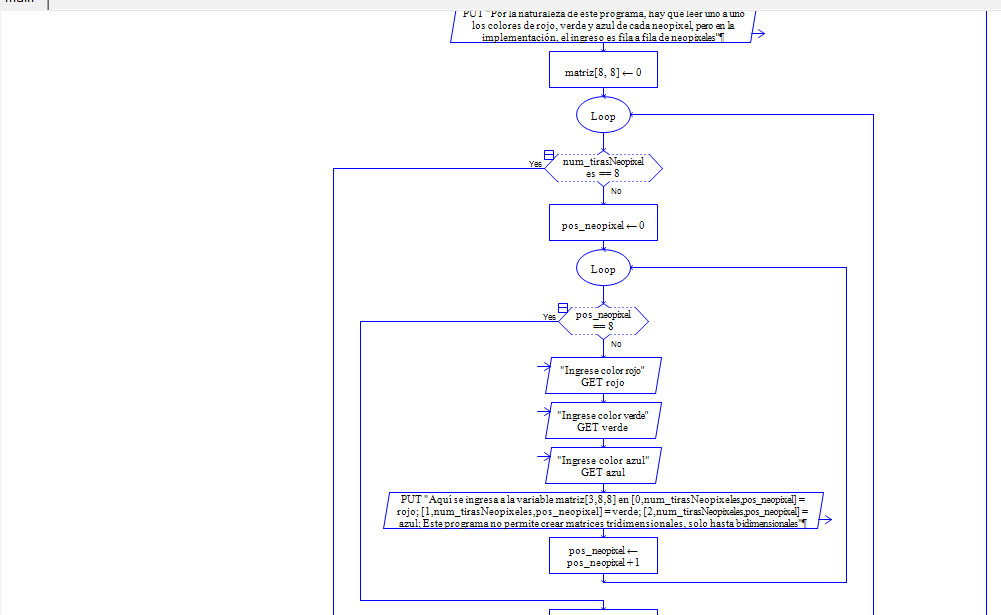
\includegraphics[width=8cm]{flow_4.png}
    \centering
    \caption{Diagrama de Flujo 4}
    \label{fig:flow_4}
 \end{figure}
  \begin{figure}[h]
    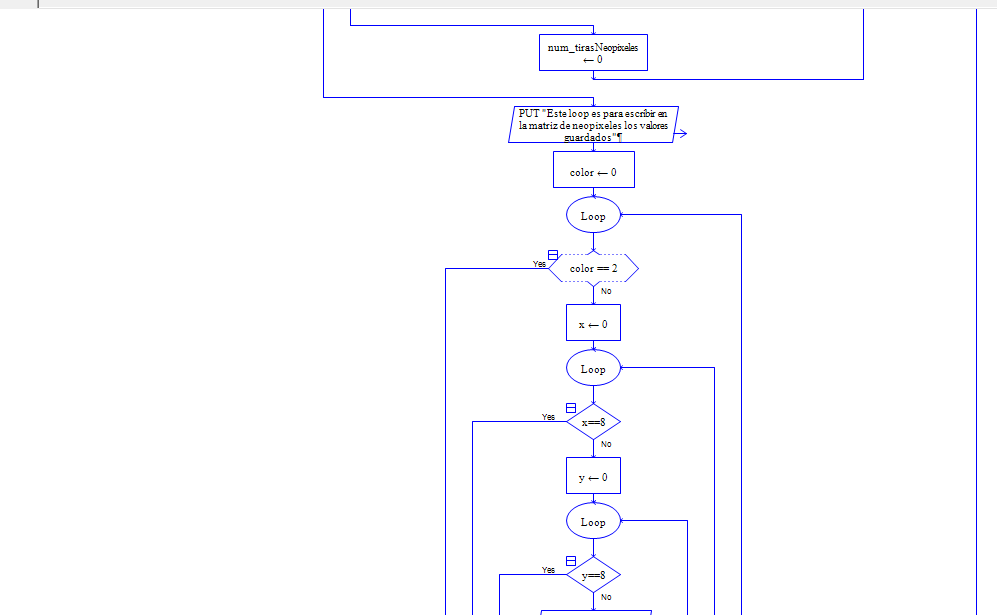
\includegraphics[width=8cm]{flow_5.png}
    \centering
    \caption{Diagrama de Flujo 5}
    \label{fig:flow_5}
 \end{figure}
  \begin{figure}[h]
    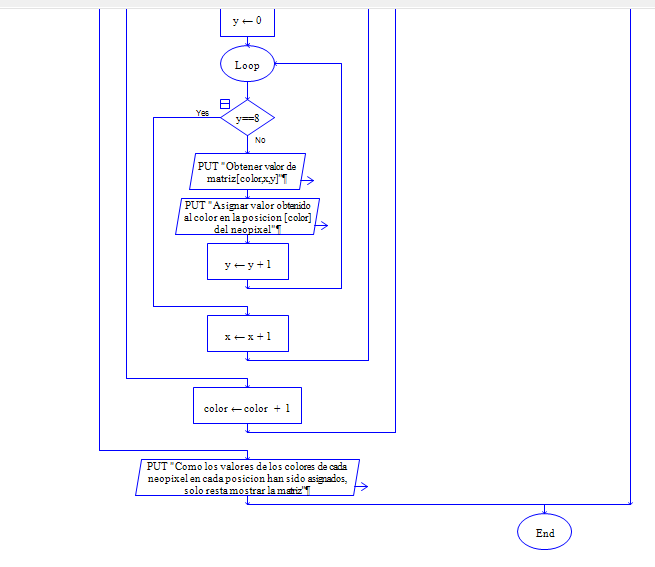
\includegraphics[width=8cm]{flow_6.png}
    \centering
    \caption{Diagrama de Flujo 6}
    \label{fig:flow_6}
 \end{figure}
 \section{Consideraciones a tener en cuenta en la implementación}
 Al analizar la alternativa de solución propuesta y su respectivo algoritmo, considero que uno de los mayores problemas en la implementación, corresponde al uso excesivo de memoria para el guardado de información de los valores enteros por color de cada pixel de la imagen, por lo cual es fundamental buscar métodos en las clases ya integradas en Qt que permitan la modificación de pixeles en la misma imagen de modo que sea innecesario el uso de memoria adicional para realizar el proceso de submuestreo o de sobremuestreo de la imagen. Dado caso de que esto no sea posible en mediana o completamente, hay que proceder al análisis de la utilidad de cada contenedor que provee C++ tanto para la parte del procesamiento de la imagen, cuyo algoritmo está planteado de modo que se fundamenta tanto en la búsqueda como modificación de los elementos de la matriz que abarca los valores enteros de rojo, verde y azul que posee la imagen; así como para las cuestiones de guardado y fácil acceso a los valores enteros finales que van a ser escritos en el archivo de texto y utilizados como referencia para configurar cada uno de los neopixeles de la matriz construida en el proyecto de Tinkercad. Otra de las consideraciones a tener en cuenta, es mantener por separadas las funciones y métodos que sean empleadas para las cuestiones de procesamiento de la imagen aparte de aquellas usadas para la creación del archivo de texto y escritura de los valores enteros dentro de la matriz, con el fin de mantener un mejor orden dentro de las funciones que cumplen los archivos que componen el proyecto en Qt. Del mismo modo, al tratarse de lógicas parecidas pero en últimas distintas, es fundamental que el análisis que conlleva el procesamiento de la imagen, cuando se emplea su sobremuestreo, sea separado por funciones del análisis que se requiera hacer un submuestreo. Por último, lo más fundamental es procurar que los elementos de la segunda clase, la que se encarga del guardado de los valores enteros finales de cada color de cada pixel, posea los elementos privados que sean útiles tanto para cumplir con su principal objetivo como aquellos que sean manejados más como herramientas auxiliares en el procesamiento de los datos de la imagen, que son obtenidos y modificados gracias a la primera clase instaurada.
\bibliographystyle{IEEEtran}
\bibliography{references}

\end{document}